\section{Dedução da Lei de Biot-Savart}

\begin{deducao}

% Figura ilustrativa
\begin{figure}[h]
\centering
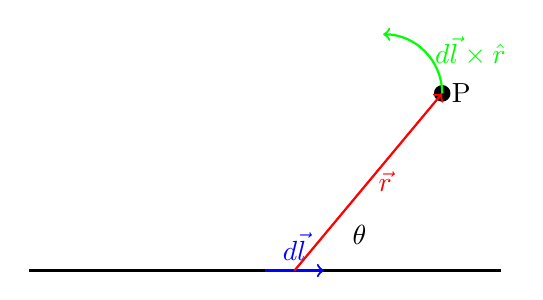
\begin{tikzpicture}[scale=1.5]
% Wire
\draw[thick] (-2,0) -- (2,0);
% dl
\coordinate (origin) at (0,0);
\coordinate (dl_end) at (0.5,0);
\coordinate (P) at (1.5,1.5);
\coordinate (r_mid) at (0.25,0);
\draw[->, blue, thick] (origin) -- (dl_end) node[midway, above] {$d\vec{l}$};
% Point P
\fill (P) circle (2pt) node[right] {P};
% r
\draw[->, red, thick] (r_mid) -- (P) node[midway, right] {$\vec{r}$};
% theta
\node at (0.8,0.3) {$\theta$};
% dl x rhat
\draw[->, green, thick] (P) arc (0:90:0.5) node[midway, right] {$d\vec{l} \times \hat{r}$};
\end{tikzpicture}
\end{figure}

% Etapa 1: Campo de uma carga puntiforme
\deducaostep[BrickRed]{Etapa 1: Campo magnético devido a uma carga puntiforme em movimento}{O campo magnético $d\vec{B}$ produzido por uma carga $q$ movendo-se com velocidade $\vec{v}$ é dado por:
\begin{align}
d\vec{B} &= \frac{\mu_0}{4\pi} \frac{q \vec{v} \times \hat{r}}{r^2}
\end{align}
onde $\hat{r}$ é o vetor unitário na direção de $\vec{r}$, o vetor do ponto de observação à carga.}

% Etapa 2: Para corrent e contínua
\deducaostep[BrickRed]{Etapa 2: Relacionando com corrente elétrica}{Considere um condutor reto carregando corrente $I$. As cargas positivas se movem com velocidade $\vec{v}$ paralela ao condutor. A densidade linear de carga é $\lambda$ (carga por unidade de comprimento).

A corrente $I$ é definida como $I = \lambda v$, onde $v = |\vec{v}|$.

Para um elemento infinitesimal $d\vec{l}$ do condutor, a carga contida é $dq = \lambda \, dl$.

O campo magnético devido a $dq$ é:
\begin{align}
d\vec{B} &= \frac{\mu_0}{4\pi} \frac{dq \, \vec{v} \times \hat{r}}{r^2} \\
&= \frac{\mu_0}{4\pi} \frac{(\lambda \, dl) \vec{v} \times \hat{r}}{r^2} \\
&= \frac{\mu_0}{4\pi} \frac{\lambda v \, d\vec{l} \times \hat{r}}{r^2}
\end{align}}

% Etapa 3: Substituir I
\deducaostep[BrickRed]{Etapa 3: Substituindo a corrente}{Como $I = \lambda v$, temos $\lambda v = I$. Substituindo:
\begin{align}
d\vec{B} &= \frac{\mu_0}{4\pi} \frac{I \, d\vec{l} \times \hat{r}}{r^2}
\end{align}}

% Etapa 4: Integração para condutor finito
\deducaostep[BrickRed]{Etapa 4: Campo total para um condutor finito}{Para um condutor finito, integre ao longo de todo o caminho do condutor:
\begin{align}
\vec{B} &= \frac{\mu_0 I}{4\pi} \int \frac{d\vec{l} \times \hat{r}}{r^2}
\end{align}

Essa é a Lei de Biot-Savart para o campo magnético devido a uma distribuição de corrente.}

\end{deducao}